%==============================================================================
%  RIVF 2026 — Selective Uncertainty-Aware LLM Routing for Phishing URL Triage
%
%  CAMERA-READY v2 (reorganized for publication clarity, 2026-11-23).
%  ALL NUMERIC VALUES ARE TAKEN FROM COMMITTED ARTIFACTS:
%    results/v2_runs/v2_main_metrics.json       (E3 composite, E9 five LLMs, E8, OOS, bootstrap)
%    results/v2_runs/v2_policies.json           (Table policies, OOF-tuned on E4)
%    results/v2_runs/v2_frontier_and_error.json (frontier, error composition, URL-Phish Cell C, single-corpus)
%    results/v2_runs/v2_paper_extras.json       (E4 check row, confusion matrices, cost)
%    results/v2_runs/oos_sample_size.json       (sign accuracy vs calibration sample size)
%    results/policies/policy_freeze_v2.json, results/policies/tau_BE_v2.json
%    results/artifacts/champion_artifact_probe.json, results/artifacts/dataset_lineage_matrix.json,
%    results/specialist_baselines/*.json, results/E3/e3_gemini_test_metrics.json (LLM latency)
%==============================================================================
\pdfminorversion=6
\documentclass[conference,a4paper]{IEEEtran}
\IEEEoverridecommandlockouts

\usepackage{cite}
\usepackage{amsmath,amssymb,amsfonts}
\usepackage{graphicx}
\usepackage{textcomp}
\usepackage{xcolor}
\usepackage{booktabs}
\usepackage{microtype}
\usepackage{url}
\usepackage{tikz}
\usetikzlibrary{shapes.geometric, arrows.meta, positioning, calc, backgrounds}

\newtheorem{proposition}{Proposition}
\newcommand{\eps}{\varepsilon}
\newcommand{\epsstar}{\eps^{\ast}}
\newcommand{\rrescue}{\rho}

\begin{document}

\title{Selective Uncertainty-Aware LLM Routing for Phishing URL
Triage: The Base-Rate Breakeven Regime and Advantage Partitioning}

\author{\IEEEauthorblockN{Jiaju Ma}
\IEEEauthorblockA{\textit{Faculty of Information Science and Technology} \\
\textit{National University of Malaysia (UKM)}\\
43600 Bangi, Selangor, Malaysia \\
FenitureMa@outlook.com, a199355@siswa.ukm.edu.my}}

\maketitle

\begin{abstract}
Escalating inputs from a fast local specialist classifier to a commercial cloud
large language model (LLM) is widely assumed to improve accuracy monotonically as
escalation budgets grow. We show that high-accuracy URL triage instead follows an
inverted-U frontier governed by a \emph{base-rate breakeven condition}: replacing
specialist verdicts with LLM verdicts yields a net gain if and only if the LLM's
error rate on specialist-correct inputs stays below $\rrescue\,E/(N-E)$, where
$E$ is the specialist error count and $\rrescue$ is the LLM rescue rate. As the
specialist strengthens, $E$ shrinks and this regression tolerance collapses. Across
$26{,}886$ test URLs from three public corpora and five commercial LLMs from four
vendors (Google, OpenAI, Anthropic, and DeepSeek), unconstrained escalation degrades
pooled detection ($-468$ net corrections, $F_1$: $0.9537\to0.9360$, exact McNemar
$p=1.39\times10^{-21}$) and helps only on the weakest specialist cohort ($+197$,
$p=2.77\times10^{-10}$). Estimated on a disjoint calibration split, the condition
predicts the test-set sign of full escalation across every corpus and the pooled
cohort. Confining escalation to the high-uncertainty head yields net gains for
every corpus and vendor. A calibration-selected threshold $\tau^{\ast}_{\mathrm{BE}}$
escalates $12.45\%$ of traffic to reach $F_1=0.9736$ ($\Delta F_1$ $95\%$ bootstrap confidence
interval (CI) $[+0.0175,+0.0221]$), cutting cloud calls by $87.55\%$ and list-price
spend from \$271 to \$33.7 per million URLs. A fixed $b=0.25$ budget similarly
reaches $F_1=0.9721$ ($\Delta F_1$ $[+0.0158,+0.0210]$) at $25.30\%$ escalation. For security
operations teams, the condition provides a pre-rollout diagnostic requiring only
$1{,}000$--$2{,}000$ labeled URLs.
\end{abstract}

\begin{IEEEkeywords}
phishing detection, model cascades, selective classification, large language
models, uncertainty estimation, cost-aware inference
\end{IEEEkeywords}

%==============================================================================
\section{Introduction}
%==============================================================================
High-throughput uniform resource locator (URL) triage in Security Operations Centers
(SOCs) and network edge appliances operates under strict latency and cost budgets. A
lexical specialist classifies a URL in well under a millisecond on a single CPU core,
whereas a commercial cloud large language model (LLM) endpoint returns in about one
second at nontrivial per-call monetary cost. The natural architecture is a two-tier cascade
(Fig.~\ref{fig:arch}) in which the local specialist resolves routine traffic
immediately and escalates only ambiguous URLs to the cloud LLM. Cascade designs
often assume that accuracy rises monotonically with escalation budget, so coverage
is capped only by latency and API spend. We show that high-accuracy binary URL triage
violates monotonicity because cloud queries past a narrow uncertainty head
degrade overall accuracy.

In a replace-on-escalation cascade, invoking an LLM on input $x$ overwrites the
specialist's verdict. On the majority of URLs that the specialist already classifies
correctly, replacement can either preserve correctness or introduce a regression. On
our pooled test cohort ($26{,}886$ URLs), the specialist already achieves $95.41\%$
accuracy, leaving only a $4.59\%$ error minority to repair. Under this base-rate
asymmetry, even a modest LLM error rate on specialist-correct inputs injects more
regressions than rescues, and the quality--cost frontier already turns downward past
roughly $20\%$ escalation.

Formulating the cascade through a \emph{base-rate breakeven condition} explains the
sign of escalation across corpora and vendors and motivates \emph{advantage
partitioning}, which restricts cloud queries to the high-uncertainty head where
rescues outnumber regressions and retains confident verdicts locally.

This paper makes four contributions:
\begin{enumerate}
\item \textbf{Base-rate breakeven condition:} We express replace-on-escalation net
gain via an explicit intrusion threshold $\epsstar = \rrescue\,E/(N-E)$, which in our
cohorts caps regression tolerance at $4.2\%$ above $95\%$ specialist accuracy.
\item \textbf{Advantage partitioning and policy comparison:} Isolating the
high-uncertainty rescue head from the confident zone reverses cascade collapse;
calibrated entropy routing matches learned deferral gates, and pairing it with soft
fusion reaches full-query fusion $F_1$ at one-quarter of the cloud cost.
\item \textbf{Out-of-sample SOC diagnostic:} Estimating $(\rrescue,\eps,\epsstar)$
on a disjoint calibration split predicts the full-escalation sign across all four
cohorts, and out-of-fold calibration selects a threshold $\tau^{\ast}_{\mathrm{BE}}$
that cuts cloud calls by $87.55\%$.
\item \textbf{Cross-vendor and error validation:} Five LLMs from Google, OpenAI,
Anthropic, and DeepSeek all lose under pooled full escalation yet gain at
$\tau^{\ast}_{\mathrm{BE}}$ in all $20$ model--cohort cells, while uncertainty
routing blocks confident-zone missed-phishing regressions. We release the offline
replay suite and response caches.
\end{enumerate}

The remainder of this paper reviews related work (Section~\ref{sec:related}),
formulates the cascade and breakeven condition (Section~\ref{sec:theory}), describes
the datasets and protocol (Section~\ref{sec:setup}), presents the empirical findings
(Section~\ref{sec:eval}), discusses deployment guidance and limitations
(Section~\ref{sec:discussion}), and concludes (Section~\ref{sec:conclusion}).

%==============================================================================
\section{Related Work}
\label{sec:related}
%==============================================================================
\subsection{Lexical and Learned URL Classifiers}
URL-only phishing detection using character $n$-grams, lexical tokenization, and
structural features with linear models, gradient-boosted trees, or neural encoders
routinely exceeds $95\%$ accuracy at sub-millisecond CPU latency~\cite{sahingoz2019,prasad2024,sahoo2019}.
This high-accuracy regime is exactly where base-rate regression tolerance tightens.
Because corpus construction can introduce single-feature artifacts~\cite{abdillah2023eval},
we audit every benchmark for lexical shortcuts prior to cascade evaluation
(Section~\ref{sec:setup}).

\subsection{LLMs for Phishing URL Triage}
Recent studies benchmark zero-shot and few-shot LLMs for phishing URL
detection~\cite{llmzeroshot2026,mdpi2025llm}, evaluate compact local language models
for cost-sensitive deployment~\cite{slm2025}, and build multi-modal agentic or hybrid
machine learning (ML)--LLM pipelines combining URL strings, HTML DOM trees, and
rendered screenshots~\cite{clasp2025,ozaslan2026}. These studies focus on expanding
LLM coverage across modalities; the base-rate conditions under which escalating URLs
from an accurate first-tier classifier triggers net system regression remain
uncharacterized.

\subsection{Selective Classification and Model Cascades}
Dynamic routing and model cascading for LLM serving use calibrated confidence scores
for cost-optimal deferral~\cite{routingsurvey2026,ucci2026} and conformal prediction
for accuracy guarantees~\cite{conformalcascade2026}, building on selective
classification and learning to defer (L2D)~\cite{geifman2017,madras2018}. Jitkrittum
et al.~\cite{jitkrittum2023} identify when confidence-based deferral is suboptimal
and derive post-hoc deferral rules. As summarized in Table~\ref{tab:relwork}, we
complement multi-class natural language processing (NLP) cascade studies by
establishing base-rate collapse,
out-of-sample breakeven prediction, and four-vendor recovery in binary security
triage above $95\%$ first-tier accuracy.

\begin{table}[!t]
\caption{Positioning relative to prior cascade and phishing triage studies.}
\label{tab:relwork}
\centering
\scriptsize
\setlength{\tabcolsep}{1.8pt}
\begin{tabular}{lllll}
\toprule
Work & Method & Sec. & Breakeven & Vendors \\
\midrule
Geifman~\cite{geifman2017}, Madras~\cite{madras2018} & Selective / L2D & No & No & No \\
Jitkrittum et al.~\cite{jitkrittum2023} & Post-hoc cascade & No & Optimal rule & No \\
UCCI~\cite{ucci2026}, Dou~\cite{conformalcascade2026} & Calib.\ / conformal & No & No & No \\
CLASP~\cite{clasp2025}, \"{O}zaslan~\cite{ozaslan2026} & Multi-modal / ML--LLM & Yes & No & No \\
\textbf{This work} & \textbf{Entropy routing + fusion} & \textbf{Yes} & \textbf{Base-rate} & \textbf{4} \\
\bottomrule
\end{tabular}
\end{table}

%==============================================================================
\section{Problem Formulation and Architecture}
\label{sec:theory}
%==============================================================================

\begin{figure}[!t]
\centering
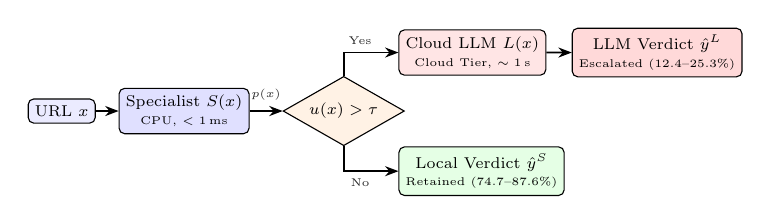
\begin{tikzpicture}[
  scale=0.81, every node/.style={transform shape},
  box/.style={draw, rectangle, rounded corners=2pt, font=\scriptsize, align=center, fill=gray!5, inner sep=3pt},
  gate/.style={draw, diamond, aspect=1.75, font=\scriptsize, align=center, fill=orange!10, inner sep=2pt},
  arr/.style={-{Stealth[scale=0.85]}, semithick},
  lbl/.style={font=\tiny, text=black!85}
]
  \node[box, fill=blue!8] (url) {URL $x$};
  \node[box, right=0.36cm of url, fill=blue!12] (spec) {Specialist $S(x)$\\{\tiny CPU, $<1\,$ms}};
  \node[gate, right=0.52cm of spec] (gate) {$u(x) > \tau$};

  \node[box, above right=0.28cm and 0.38cm of gate, fill=red!10] (llm) {Cloud LLM $L(x)$\\{\tiny Cloud Tier, $\sim 1\,$s}};
  \node[box, below right=0.28cm and 0.38cm of gate, fill=green!10] (local) {Local Verdict $\hat{y}^S$\\{\tiny Retained (74.7--87.6\%)}};
  \node[box, right=0.40cm of llm, fill=red!15] (llm_out) {LLM Verdict $\hat{y}^L$\\{\tiny Escalated (12.4--25.3\%)}};

  \draw[arr] (url) -- (spec);
  \draw[arr] (spec) -- node[above=1pt, lbl] {$p(x)$} (gate);
  \draw[arr] (gate) |- node[above, pos=0.65, lbl] {Yes} (llm);
  \draw[arr] (gate) |- node[below, pos=0.65, lbl] {No} (local);
  \draw[arr] (llm) -- (llm_out);
\end{tikzpicture}
\caption{Two-tier uncertainty-aware URL triage cascade. The local specialist resolves
low-entropy URLs ($74.7\%$--$87.6\%$ of traffic) on CPU in under $1\,$ms and escalates
only inputs with $u(x)>\tau$ ($12.4\%$--$25.3\%$) to the cloud LLM, isolating rescues
while blocking confident-zone regressions.}
\label{fig:arch}
\end{figure}

\subsection{Cascade and Routing Policy}
Let $\mathcal{D}=\{(x_i,y_i)\}_{i=1}^{N}$ denote a set of URLs with ground-truth
labels $y_i\in\{0,1\}$, where $1$ indicates phishing. As shown in Fig.~\ref{fig:arch},
a specialist classifier $S$ outputs a binary verdict $\hat{y}^S_i$ and calibrated
posterior $p_i = \Pr(y_i=1 \mid x_i)$. An uncertainty router computes binary Shannon
entropy $u_i = -p_i \log_2 p_i - (1-p_i) \log_2 (1-p_i)$ and escalates the
high-uncertainty subset
\begin{equation}
\mathcal{U}(\tau) = \{i : u_i > \tau\}
\label{eq:topzone}
\end{equation}
to a cloud-hosted LLM $L$, which returns verdict $\hat{y}^L_i$. Under
replace-on-escalation, the cascade outputs
\begin{equation}
\hat{y}_i =
\begin{cases}
\hat{y}^L_i, & i \in \mathcal{U}(\tau),\\[2pt]
\hat{y}^S_i, & i \in \mathcal{U}^c(\tau),
\end{cases}
\label{eq:cascade}
\end{equation}
where $\mathcal{U}^c(\tau)=\mathcal{D}\setminus\mathcal{U}(\tau)$ is the retained
confident zone. Malformed responses or endpoint failures fall back deterministically
to $\hat{y}^S_i$ in~\eqref{eq:cascade}.

\begin{figure}[!t]
\centering
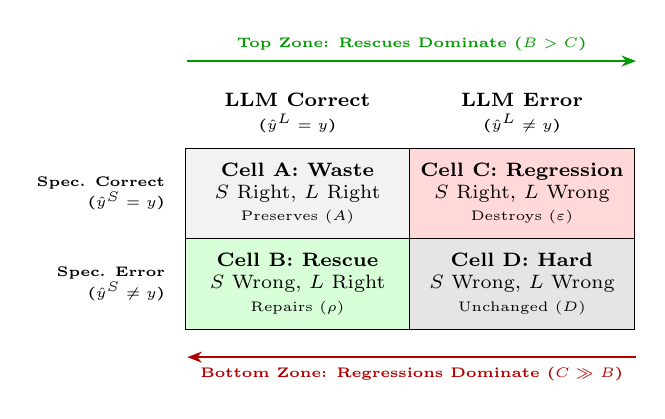
\begin{tikzpicture}[
  every node/.style={font=\scriptsize},
  cell/.style={draw, rectangle, minimum width=2.85cm, minimum height=1.15cm,
               align=center, inner sep=2pt}
]
  \node[cell, fill=gray!10]  (A) at (0,0)        {\textbf{Cell A: Waste}\\$S$ Right, $L$ Right\\{\tiny Preserves ($A$)}};
  \node[cell, fill=red!15]   (C) at (2.85,0)     {\textbf{Cell C: Regression}\\$S$ Right, $L$ Wrong\\{\tiny Destroys ($\eps$)}};
  \node[cell, fill=green!15] (B) at (0,-1.15)    {\textbf{Cell B: Rescue}\\$S$ Wrong, $L$ Right\\{\tiny Repairs ($\rrescue$)}};
  \node[cell, fill=gray!20]  (D) at (2.85,-1.15) {\textbf{Cell D: Hard}\\$S$ Wrong, $L$ Wrong\\{\tiny Unchanged ($D$)}};

  \node[font=\scriptsize\bfseries, align=center] at (0,1.02)    {LLM Correct\\{\tiny ($\hat{y}^L = y$)}};
  \node[font=\scriptsize\bfseries, align=center] at (2.85,1.02) {LLM Error\\{\tiny ($\hat{y}^L \ne y$)}};

  \node[font=\tiny\bfseries, align=right, anchor=east] at (-1.56,0)     {Spec. Correct\\($\hat{y}^S = y$)};
  \node[font=\tiny\bfseries, align=right, anchor=east] at (-1.56,-1.15) {Spec. Error\\($\hat{y}^S \ne y$)};

  \draw[thick, green!60!black, -{Stealth[scale=0.8]}] (-1.40,1.68) --
    node[above, font=\tiny\bfseries] {Top Zone: Rescues Dominate ($B > C$)} (4.30,1.68);
  \draw[thick, red!70!black, -{Stealth[scale=0.8]}] (4.30,-2.08) --
    node[below, font=\tiny\bfseries] {Bottom Zone: Regressions Dominate ($C \gg B$)} (-1.40,-2.08);
\end{tikzpicture}
\caption{Four-quadrant rescue--regression taxonomy. Net cascade gain is
$\Delta_{\mathrm{net}} = |B| - |C|$; uncertainty routing isolates Cell B in the Top
Zone while blocking Cell C regressions in the Bottom Zone.}
\label{fig:taxonomy}
\end{figure}

\subsection{Rescue--Regression Taxonomy}
Every URL falls into one cell of the $2\times2$ outcome taxonomy
(Fig.~\ref{fig:taxonomy}): A ($S$ and $L$ right; wasted cloud spend, $0$), B ($S$ wrong,
$L$ right; a \emph{rescue}, $+1$), C ($S$ right, $L$ wrong; a \emph{regression}, $-1$),
or D (both wrong; $0$).
With total specialist error count $E = |B| + |D|$, escalating any subset
$Z \subseteq \mathcal{D}$ changes the number of correct predictions by
\begin{equation}
\Delta_{\mathrm{net}}(Z) = |B \cap Z| - |C \cap Z|.
\label{eq:delta}
\end{equation}

\subsection{Base-Rate Breakeven Condition and Partitioning}
For any cohort with $0 < E < N$, define the LLM \emph{rescue rate} on specialist
errors as $\rrescue = |B|/E$ and its \emph{intrusion rate} on specialist-correct
inputs as $\eps = |C|/(N-E)$.

\begin{proposition}[Base-Rate Breakeven Condition]
\label{thm:breakeven}
Under full escalation ($Z=\mathcal{D}$) with $0 < E < N$,
\begin{equation}
\Delta_{\mathrm{net}} = \rrescue E - \eps(N{-}E) > 0 \iff \eps < \epsstar \triangleq \rrescue\frac{E}{N{-}E}.
\label{eq:breakeven}
\end{equation}
\end{proposition}
\begin{IEEEproof}
Substituting $|B|=\rrescue E$ and $|C|=\eps(N-E)$ into~\eqref{eq:delta} with
$Z=\mathcal{D}$ yields~\eqref{eq:breakeven}; when $E=0$,
$\Delta_{\mathrm{net}}=-|C|\le 0$.
\end{IEEEproof}
Proposition~\ref{thm:breakeven} is an exact accounting identity on the $2\times2$
outcome table; its operational value is prospective, because $(\rrescue,\eps)$
estimated on a small calibration sample diagnoses whether escalation helps \emph{before}
rollout (Section~\ref{sec:eval}).
Expressed via the specialist error base rate $\pi = E/N \in (0, 1)$,
\begin{equation}
\epsstar = \rrescue\,\frac{\pi}{1-\pi}.
\label{eq:baserate}
\end{equation}
As the specialist strengthens ($\pi \to 0$), the repairable pool $E$ shrinks relative
to the regression-vulnerable majority $N-E$, driving the tolerable intrusion rate
$\epsstar \to 0$.

Applying the same condition locally to any escalated region $Z \subseteq \mathcal{D}$
with $N_Z = |Z| > 0$ and $E_Z \in (0, N_Z)$ gives
\begin{equation}
\Delta_{\mathrm{net}}(Z) > 0 \iff \eps_Z < \rrescue_Z\,\frac{E_Z}{N_Z - E_Z}.
\label{eq:local_breakeven}
\end{equation}
Uncertainty routing partitions $\mathcal{D}$ into a high-uncertainty \emph{Top Zone}
$\mathcal{U}(\tau)$ in~\eqref{eq:topzone} and a confident \emph{Bottom Zone}
$\mathcal{U}^c(\tau)$. Inside $\mathcal{U}(\tau)$, specialist errors concentrate
($\pi_{\mathcal{U}} \gg \pi$), lifting $\epsstar_{\mathcal{U}}$ well above
$\eps_{\mathcal{U}}$ while preventing regressions in the Bottom Zone.

%==============================================================================
\section{Experimental Setup and Leakage Control}
\label{sec:setup}
%==============================================================================
\subsection{Corpora and Shortcut Auditing}
We evaluate across three public URL corpora spanning distinct collection eras:
\textbf{PWD2021}~\cite{ariyadasa2021dataset} ($N_{\mathrm{test}}=11{,}564$),
\textbf{EBBU2017}~\cite{sahingoz2019} ($N_{\mathrm{test}}=8{,}784$), and
\textbf{URL-Phish 2025}~\cite{linh2025dataset} ($N_{\mathrm{test}}=6{,}538$),
totaling $26{,}886$ balanced test URLs drawn from
$134{,}446$ per-corpus deduplicated manifest URLs. Table~\ref{tab:corpora} audits single-feature shortcuts
($|\text{acc} - 0.5|$ for path presence, URL scheme, and cross-validated top-level
domain (TLD) lookups): URL-Phish~2025 exhibits the strongest scheme ($0.286$) and TLD ($0.811$)
regularities, whereas PWD2021 and EBBU2017 are substantially more balanced. Because
the PWD2021 and EBBU2017 manifests share $4{,}835$ canonical URLs ($11.0\%$ of
EBBU2017; at most $18$ for any other corpus pair), we report both per-corpus results
and a strict single-corpus sensitivity check ($N=24{,}921$).

\begin{table}[!t]
\caption{Corpora and single-feature shortcut audit (balanced {\upshape\texttt{TEST}}
splits; majority-class baseline $=0.5000$).}
\label{tab:corpora}
\centering
\scriptsize
\setlength{\tabcolsep}{3.0pt}
\begin{tabular}{lrrrrr}
\toprule
Corpus & $N_{\mathrm{test}}$ & Path $|{\cdot}{-}0.5|$ & Scheme $|{\cdot}{-}0.5|$
& TLD acc & TLD $F_1$ \\
\midrule
PWD2021      & 11{,}564 & 0.068 & 0.148 & 0.644 & 0.515 \\
EBBU2017     &  8{,}784 & 0.015 & 0.169 & 0.653 & 0.538 \\
URL-Phish 25 &  6{,}538 & 0.159 & 0.286 & 0.811 & 0.823 \\
\bottomrule
\end{tabular}
\end{table}

\begin{table}[!t]
\caption{Traditional URL-classifier baselines on {\upshape\texttt{TEST}}
($F_1$, mean $\pm$ std over ten random split seeds).}
\label{tab:baselines}
\centering
\scriptsize
\setlength{\tabcolsep}{1.6pt}
\begin{tabular}{lccc}
\toprule
First-tier model & PWD2021 & EBBU2017 & URL-Phish 25 \\
\midrule
Char TF--IDF $+$ LogReg$^{\mathrm{a}}$ & $0.9363{\pm}0.0018$ & $0.9660{\pm}0.0012$ & $0.9755{\pm}0.0016$ \\
Char TF--IDF $+$ LinearSVM             & $0.9463{\pm}0.0013$ & $0.9767{\pm}0.0012$ & $0.9805{\pm}0.0017$ \\
Char TF--IDF $+$ Na\"{\i}ve Bayes      & $0.9175{\pm}0.0024$ & $0.9593{\pm}0.0023$ & $0.9546{\pm}0.0028$ \\
Lexical $+$ XGBoost                    & $0.7876{\pm}0.0023$ & $0.7709{\pm}0.0049$ & $0.8867{\pm}0.0039$ \\
Lexical $+$ Random Forest              & $0.7872{\pm}0.0033$ & $0.7643{\pm}0.0056$ & $0.8935{\pm}0.0026$ \\
\bottomrule
\end{tabular}\\[2pt]
{\scriptsize $^{\mathrm{a}}$Adopted as the cascade first tier.}
\end{table}

\begin{table*}[!t]
\caption{Base-rate breakeven validation and advantage partitioning across corpora and
five commercial LLMs. $\epsstar=\rrescue\,E/(N{-}E)$ (Proposition~\ref{thm:breakeven});
Top Zone $\mathcal{U}(\tau)=\{u_i>\tau\}$, Bottom Zone its complement. Primary fixed
budget $\tau=0.1997$ ($b=0.25$); calibration-selected $\tau^{\ast}_{\mathrm{BE}}=0.4567$.}
\label{tab:breakeven}
\centering
\scriptsize
\setlength{\tabcolsep}{3.6pt}
\begin{tabular}{lrrrrrrrrr}
\toprule
& & Spec. & Rescue & Breakeven & Measured & Full escalation & \multicolumn{2}{c}{Primary $\tau$ ($b{=}0.25$)} & $\tau^{\ast}_{\mathrm{BE}}$ \\
\cmidrule(lr){8-9}\cmidrule(lr){10-10}
Cohort (model) & $N$ & acc. & $\rrescue$ & $\epsstar$ & $\eps$ &
$\Delta_{\mathrm{net}}$ (McNemar $p$) & Top (\% esc.) & Bottom & Top (\% esc.) \\
\midrule
PWD2021 (Gemini) & 11{,}564 & 93.48\% & 77.45\% & 5.40\% & \textbf{3.58\%} & $+197$ \ ($2.77\times10^{-10}$) & $+312$ \ (34.1\%) & $-115$ & $+320$ \ (20.1\%) \\
EBBU2017 (Gemini) & 8{,}784 & 96.55\% & 78.88\% & 2.82\% & 3.75\% & $-79$ \ ($9.33\times10^{-4}$) & $+84$ \ (19.6\%) & $-163$ & $+119$ \ (7.4\%) \\
URL-Phish 25 (Gemini) & 6{,}538 & 97.29\% & 83.62\% & 2.33\% & 11.54\% & $-586$ \ ($5.36\times10^{-94}$) & $+89$ \ (17.3\%) & $-675$ & $+85$ \ (5.5\%) \\
\midrule
\textbf{Pooled E3 \texttt{TEST}} & 26{,}886 & 95.41\% & 78.69\% & 3.79\% & 5.61\% & $-468$ \ ($1.39\times10^{-21}$) & $+485$ \ (25.3\%) & $-953$ & $+524$ \ (12.4\%) \\
E4 \texttt{CAL} check$^{\mathrm{b}}$ & 13{,}261 & 95.55\% & 78.64\% & 3.66\% & 5.87\% & $-280$ \ ($7.44\times10^{-16}$) & $+235$ \ (25.4\%) & $-515$ & $+259$ \ (12.7\%) \\
\midrule
E9: Gemini 3.5 Flash-Lite & 3{,}000 & 95.17\% & 82.07\% & 4.17\% & 6.58\% & $-69$ \ ($9.78\times10^{-5}$) & $+75$ \ (24.6\%) & $-144$ & $+75$ \ (11.3\%) \\
E9: GPT-5.6 Luna & 3{,}000 & 95.17\% & 77.24\% & 3.92\% & 9.67\% & $-164$ \ ($4.34\times10^{-17}$) & $+52$ \ (24.6\%) & $-216$ & $+63$ \ (11.3\%) \\
E9: GPT-6 Luna & 3{,}000 & 95.17\% & 73.79\% & 3.75\% & 9.46\% & $-163$ \ ($2.27\times10^{-17}$) & $+40$ \ (24.6\%) & $-203$ & $+54$ \ (11.3\%) \\
E9: DeepSeek-V4.1-Flash & 3{,}000 & 95.17\% & 68.28\% & 3.47\% & 9.98\% & $-186$ \ ($5.50\times10^{-22}$) & $+24$ \ (24.6\%) & $-210$ & $+42$ \ (11.3\%) \\
E9: Claude Haiku 5.5 & 3{,}000 & 95.17\% & 75.86\% & 3.85\% & 8.41\% & $-130$ \ ($3.04\times10^{-12}$) & $+46$ \ (24.6\%) & $-176$ & $+58$ \ (11.3\%) \\
\bottomrule
\end{tabular}\\[2pt]
{\scriptsize $^{\mathrm{b}}$Calibration split (\texttt{CAL\_ROUTER}) with in-sample isotonic scores; $185$ cross-split URLs excluded.}
\end{table*}

\subsection{Partitions and Leakage Control}
Table~\ref{tab:baselines} benchmarks five standard first-tier URL classifiers over
ten random seeds. On every corpus, the best character $3$--$5$-gram term
frequency--inverse document frequency (TF--IDF) model
outperforms the best hand-crafted lexical tree model by $8.7$--$20.6$ $F_1$ points;
we adopt logistic regression (LogReg) as the first tier for its native probability
posteriors and near-peak TF--IDF accuracy (seed-42 pooled test accuracy $0.9541$,
$F_1$ $0.9537$, Matthews correlation coefficient (MCC) $0.9083$).

Each corpus is partitioned $60/10/10/20$ into disjoint \texttt{TRAIN} /
\texttt{CAL\_ROUTER} / \texttt{DEV\_POLICY} / \texttt{TEST} splits under per-corpus
canonical-URL hash isolation. Specialists are trained exclusively on \texttt{TRAIN}
and isotonically calibrated on \texttt{CAL\_ROUTER}. To prevent cross-corpus leakage
during parameter estimation, all $185$ \texttt{CAL\_ROUTER} URLs that appear in
another corpus's \texttt{TEST} split are excluded from every calibration estimate
($N_{\mathrm{E4}}=13{,}261$).

We evaluate two operating points, both selected without \texttt{TEST} labels:
\begin{enumerate}
\item \textbf{Fixed-budget threshold $\tau=0.1997$:} the $(1-b)$ quantile of
calibrated bit-entropy on \texttt{DEV\_POLICY} at nominal budget $b=0.25$ (escalating
$24.94\%$ on \texttt{DEV\_POLICY} and $25.30\%$ on \texttt{TEST}).
\item \textbf{Breakeven-optimal threshold $\tau^{\ast}_{\mathrm{BE}}=0.4567$:}
maximizes net gain $B-C$ on \texttt{CAL\_ROUTER} using five-fold out-of-fold
isotonic probabilities ($2{,}000$-resample $95\%$ bootstrap confidence interval (CI)
$[0.276, 0.545]$) and transfers unchanged to \texttt{TEST} ($12.45\%$ escalation).
\end{enumerate}

\subsection{LLM Protocol and Cross-Vendor Cohort}
Run IDs E3 (\texttt{TEST}), E4 (\texttt{CAL\_ROUTER}), and E9 (five-LLM \texttt{TEST}
subset) index our cached evaluations, distinct from error count $E$.
The primary second-tier model is Google Gemini~3.5 Flash-Lite, queried with
\texttt{temperature=0}, \texttt{topP=1}, minimal thinking, and a JSON response
schema. Of the $26{,}886$ E3 rows, $23{,}273$ were answered in August~2026 via the
\texttt{gemini-flash-lite-latest} alias (server-reported version
\texttt{gemini-3.5-flash-lite}) and $3{,}605$ in November~2026 via the pinned ID;
$8$ empty responses fall back to $S$. Two stability probes quantify temporal and
decoding consistency: a $1{,}000$-URL cross-period bridge achieves $99.2\%$ verdict
agreement, and a $200\text{-URL}\times 5\text{-repeat}$ probe observes verdict flips
on $3.5\%$ of URLs, confined exclusively to the high-entropy stratum ($7\%$ vs.\
$0\%$ in the random stratum).

To test vendor generality, the shared cross-model cohort (E9) evaluates a fixed,
class-balanced $3{,}000$-row subset of \texttt{TEST} ($1{,}000$ per corpus;
$2{,}993$ unique URLs) across five production cost-efficient tiers matched to
high-throughput SOC budgets: Gemini~3.5 Flash-Lite, GPT-5.6 Luna and GPT-6 Luna
(\texttt{reasoning\_effort=medium}, JSON mode), DeepSeek-V4.1-Flash (non-thinking,
\texttt{temperature=0}, API alias \texttt{deepseek-flash}), and Claude Haiku~5.5
(low effort, thinking disabled, no temperature parameter, structured outputs; $15$
schema failures fall back to $S$). Every model receives only the canonicalized URL under one frozen,
content-hashed zero-shot prompt (\texttt{e67d6cb3\ldots8797d8d3}) without metadata
or specialist outputs, returning a verdict, probability, and 1--3 lexical signals.
All request ledgers, configuration hashes, and offline replay scripts are archived
in the public repository.

%==============================================================================
\section{Empirical Evaluation}
\label{sec:eval}
%==============================================================================



\subsection{Base-Rate Breakeven Regime and Out-of-Sample Prediction}
Full escalation across pooled E3 ($N=26{,}886$) produces $|A|=24{,}213$, $|B|=971$,
$|C|=1{,}439$, and $|D|=263$, degrading detection by $\Delta_{\mathrm{net}}=-468$
and lowering $F_1$ from $0.9537$ to $0.9360$ (exact McNemar
$p=1.39\times10^{-21}$).

On \texttt{TEST},~\eqref{eq:breakeven} reproduces each cohort's sign by construction;
what varies empirically across corpora is which regime of~\eqref{eq:baserate} holds
(Table~\ref{tab:breakeven}, Fig.~\ref{fig:breakeven_regime}). On \textbf{PWD2021}
($93.48\%$ specialist accuracy), the wide tolerance $\epsstar=5.40\%$ exceeds
$\eps=3.58\%$, yielding $+197$ net rescues ($p=2.77\times10^{-10}$). On
\textbf{EBBU2017} ($96.55\%$) and \textbf{URL-Phish~2025} ($97.29\%$), higher
first-tier accuracy compresses $\epsstar$ to $2.82\%$ and $2.33\%$, below
$\eps=3.75\%$ and $11.54\%$, yielding $\Delta_{\mathrm{net}}=-79$ and $-586$.

Out-of-sample calibration estimates predict this regime shift prior to test
evaluation. Estimating $(\hat{\rrescue},\hat{\eps},\hat{\eps}^{\ast})$ on the
disjoint calibration split E4 ($N=13{,}261$) correctly predicts the E3 \texttt{TEST}
escalation sign on $4/4$ cohorts: PWD2021
($\hat{\eps}=3.80\%<\hat{\eps}^{\ast}=5.19\%\to+$), EBBU2017
($3.71\%>2.72\%\to-$), URL-Phish~2025 ($12.18\%>2.33\%\to-$), and pooled
($5.87\%>3.66\%\to-$). Drawing $1{,}000$ random E4 subsamples of size $m$ (without
replacement) quantifies calibration sample requirements: pooled sign accuracy reaches
$0.813$ at $m=100$, $0.941$ at $m=500$, $0.989$ at $m=1{,}000$, and $1.000$ at
$m=2{,}000$; individual corpora reach $0.930$ (PWD2021), $0.918$ (EBBU2017), and
$1.000$ (URL-Phish~2025) at $m=1{,}000$, rising to $0.994$, $0.990$, and $1.000$ at
$m=2{,}000$.

\begin{figure}[!t]
\centering
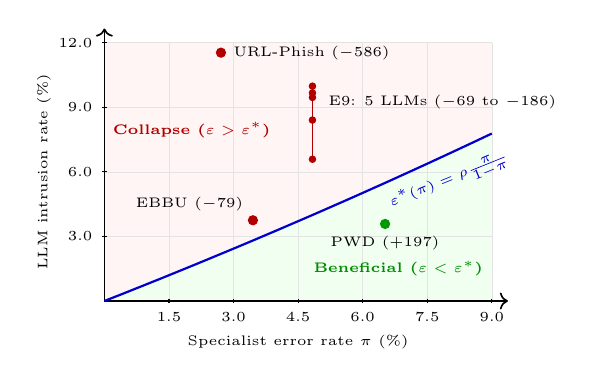
\begin{tikzpicture}[scale=0.82, every node/.style={font=\scriptsize}]
  % Regime shading clipped to plot area
  \begin{scope}
    \clip (0,0) rectangle (6.0,4.0);
    \fill[red!4] (0,4.0) -- (6.0,4.0) --
      plot[domain=6.0:0, samples=40] (\x, {(\x * 1.5 / 100) / (1 - (\x * 1.5 / 100)) * 78.69 / 3.0}) -- cycle;
    \fill[green!6] (0,0) -- (6.0,0) --
      plot[domain=6.0:0, samples=40] (\x, {(\x * 1.5 / 100) / (1 - (\x * 1.5 / 100)) * 78.69 / 3.0}) -- cycle;
  \end{scope}

  % Grid & Axes
  \draw[help lines, color=gray!22, step=1.0cm] (0,0) grid (6.0,4.0);
  \draw[->, semithick] (0,0) -- (6.25,0);
  \draw[->, semithick] (0,0) -- (0,4.22);

  % Axis ticks & titles
  \foreach \x/\val in {1/1.5, 2/3.0, 3/4.5, 4/6.0, 5/7.5, 6/9.0}
    \draw (\x,1pt) -- (\x,-1pt) node[below, font=\tiny] {\val};
  \foreach \y/\val in {1/3.0, 2/6.0, 3/9.0, 4/12.0}
    \draw (1pt,\y) -- (-1pt,\y) node[left, font=\tiny] {\val};
  \node[below, font=\tiny] at (3.0,-0.38) {Specialist error rate $\pi$ (\%)};
  \node[above, rotate=90, font=\tiny] at (-0.68,2.0) {LLM intrusion rate (\%)};

  % Breakeven Curve eps* = rho * pi / (1 - pi), pooled rho = 0.7869
  \draw[thick, blue!80!black, domain=0:6.0, samples=50] plot (\x, {(\x * 1.5 / 100) / (1 - (\x * 1.5 / 100)) * 78.69 / 3.0});
  \node[font=\tiny\bfseries, blue!80!black, rotate=22] at (5.35, 1.85) {$\epsstar(\pi) = \rrescue \frac{\pi}{1-\pi}$};

  % Regions
  \node[font=\tiny\bfseries, green!55!black] at (4.55, 0.50) {Beneficial ($\eps < \epsstar$)};
  \node[font=\tiny\bfseries, red!70!black] at (1.35, 2.65) {Collapse ($\eps > \epsstar$)};

  % Empirical points (x = pi/1.5, y = eps/3)
  \filldraw[green!60!black] (4.347, 1.193) circle (2pt) node[below=1pt, font=\tiny, black] {PWD ($+197$)};
  \filldraw[red!70!black] (2.300, 1.250) circle (2pt) node[above left, font=\tiny, black] {EBBU ($-79$)};
  \filldraw[red!70!black] (1.805, 3.846) circle (2pt) node[right=1pt, font=\tiny, black] {URL-Phish ($-586$)};
  % E9 subset, five LLMs (same specialist, pi = 4.83%)
  \draw[red!70!black, thin] (3.222, 2.195) -- (3.222, 3.327);
  \foreach \y in {2.195, 2.802, 3.152, 3.222, 3.327}
    \filldraw[red!70!black] (3.222, \y) circle (1.4pt);
  \node[font=\tiny, black, anchor=west] at (3.32, 3.08) {E9: 5 LLMs ($-69$ to $-186$)};
\end{tikzpicture}
\caption{Base-rate breakeven boundary~\eqref{eq:baserate} (plotted at pooled $\rrescue=78.69\%$). As
specialist error $\pi$ declines, tolerable intrusion $\epsstar$ collapses; every
plotted cohort above the curve degrades under full escalation.}
\label{fig:breakeven_regime}
\end{figure}

\subsection{Advantage Partitioning Across Cohorts}
Restricting escalation to the high-uncertainty head reverses collapse in every
corpus (Table~\ref{tab:breakeven}), as the local condition~\eqref{eq:local_breakeven}
predicts. At the fixed-budget threshold $\tau=0.1997$,
escalating $25.30\%$ of pooled E3 traffic recovers $+485$ net corrections ($B=899$,
$C=414$), lifting $F_1$ from $0.9537$ to $0.9721$ ($\Delta F_1$ $95\%$ paired bootstrap CI
$[+0.0158,+0.0210]$); escalating the remaining $74.70\%$ confident zone would add a net $-953$. Every corpus gains significantly: PWD2021 $0.9343\to0.9620$
($[+0.0229,+0.0325]$), EBBU2017 $0.9654\to0.9749$ ($[+0.0053,+0.0137]$), and
URL-Phish~2025 $0.9725\to0.9865$ ($[+0.0099,+0.0181]$).

The calibration-selected $\tau^{\ast}_{\mathrm{BE}}$ halves escalation ($12.45\%$)
and raises net rescues to $+524$ ($B=759$, $C=235$; $F_1=0.9736$, $\Delta F_1$ CI
$[+0.0175,+0.0221]$). Both the $24{,}921$ single-corpus URLs (specialist
$F_1=0.9560$, full escalation $0.9382$ at $-469$, $\tau$ $0.9736$ at $+462$ and
$25.70\%$, $\tau^{\ast}_{\mathrm{BE}}$ $0.9752$ at $+504$ and $12.56\%$) and the E4
calibration split ($N=13{,}261$: $-280$ full, $+235$ at $\tau$, $+259$ at
$\tau^{\ast}_{\mathrm{BE}}$) exhibit the same partitioning gain.

\subsection{Budget Frontier, Calibration, and Policy Alternatives}
Table~\ref{tab:frontier} and Fig.~\ref{fig:frontier} map the inverted-U frontier:
$F_1$ rises from $0.9537$ to a ridge at $10\%$--$20\%$ escalation
($0.9735$--$0.9741$), then falls to $0.9619$ at $50.38\%$ and $0.9360$ at $100\%$. Beyond the isotonic zero-entropy
plateau ($79.23\%$, $+10$), the final $20.8\%$ of URLs adds just $1$ rescue against
$479$ regressions. Over full escalation, selective routing improves $F_1$ by
$[+0.0338,+0.0387]$ at $\tau$ and $[+0.0349,+0.0404]$ at $\tau^{\ast}_{\mathrm{BE}}$
($10{,}000$ paired bootstrap resamples), whereas random $25\%$ routing degrades $F_1$
to $0.9476$ ($-159$).

\subsubsection{Ranking Equivalence and Calibration}
For binary posteriors $p$, Shannon entropy, $\max(p,1-p)$, margin $|2p-1|$, and
conformal nonconformity $1-\max(p,1-p)$ are strictly monotone in $|p-0.5|$ and
induce identical uncertainty orderings.
At matched $12.45\%$ escalation (Table~\ref{tab:policies}), per-corpus temperature
scaling ($F_1=0.9736$, $+526$) and isotonic calibration ($0.9736$, $+524$) both
outperform uncalibrated entropy ($0.9732$, $+517$), with isotonic calibration
retaining the edge at $25.30\%$ ($0.9721$ vs.\ $0.9716$ and $0.9713$).

\subsubsection{Policy-Space Comparison}
Table~\ref{tab:policies} compares alternative deferral rules tuned on E4:
(i)~\emph{Confidence-gated override} ($\max(p_L,1-p_L)\ge c_L$) avoids full-query
collapse only by suppressing nearly all overrides: tuned $c_L=0.99$ eliminates
$99\%$ of regressions ($C=10$) at the expense of $98\%$ of rescues ($B=20$,
$F_1=0.9541$).
(ii)~\emph{Soft fusion} ($0.5\,p_S+0.5\,p_L$) reaches $F_1=0.9748$ at $100\%$
querying, yet restricting the same fusion to the $25.30\%$ primary Top Zone achieves
the identical $F_1=0.9748$ ($C$ cut from $414$ to $218$): high-confidence specialist
posteriors are rarely overturned by averaging.
(iii)~\emph{Learned gates}~\cite{jitkrittum2023} trained to predict $P(B|x)>P(C|x)$
on E4 reach $F_1=0.9739$ with LogReg ($14.46\%$) and $0.9736$ with histogram gradient
boosting (HGB, $14.25\%$), matching the entropy ridge.

\begin{table}[!t]
\caption{Routing frontier of the entropy router on E3 ($N=26{,}886$). Nominal $b$ is
the {\upshape\texttt{DEV\_POLICY}} quantile budget under strict routing ($u_i>\tau$);
$b=0.80$--$0.95$ share one threshold at the isotonic zero-entropy plateau. Net
rescue rate $\text{NRR}_{\mathrm{esc}}=\Delta_{\mathrm{net}}/\#\text{escalated}$.}
\label{tab:frontier}
\centering
\scriptsize
\setlength{\tabcolsep}{2.3pt}
\begin{tabular}{lrrrrrrr}
\toprule
Nom.\ $b$ & Esc.\ \% & $B$ & $C$ & $\Delta_{\mathrm{net}}$ & $\text{NRR}_{\mathrm{esc}}$ & $F_1$ & $\Delta F_1$ \\
\midrule
0.00 (Spec) & 0.00 & 0 & 0 & 0 & --- & 0.9537 & $0.0000$ \\
0.05 & 4.53 & 409 & 80 & $+329$ & $+27.0\%$ & 0.9661 & $+0.0124$ \\
0.10 & 10.47 & 709 & 187 & $+522$ & $+18.5\%$ & 0.9735 & $+0.0197$ \\
$\tau^{\ast}_{\mathrm{BE}}$ & 12.45 & 759 & 235 & $+524$ & $+15.7\%$ & 0.9736 & $+0.0198$ \\
0.15 & 14.14 & 798 & 268 & $+530$ & $+13.9\%$ & 0.9738 & $+0.0201$ \\
0.20 (peak) & 19.85 & 869 & 332 & $+537$ & $+10.1\%$ & 0.9741 & $+0.0204$ \\
\textbf{0.25 ($\tau$)} & \textbf{25.30} & \textbf{899} & \textbf{414} & $\mathbf{+485}$ & $\mathbf{+7.1\%}$ & \textbf{0.9721} & $\mathbf{+0.0184}$ \\
0.35 & 37.10 & 937 & 558 & $+379$ & $+3.8\%$ & 0.9683 & $+0.0146$ \\
0.50 & 50.38 & 953 & 746 & $+207$ & $+1.5\%$ & 0.9619 & $+0.0082$ \\
0.80--0.95 & 79.23 & 970 & 960 & $+10$ & $+0.0\%$ & 0.9548 & $+0.0010$ \\
1.00 (Full) & 100.00 & 971 & 1{,}439 & $-468$ & $-1.7\%$ & 0.9360 & $-0.0178$ \\
\midrule
Random 0.25 & 25.14 & 228 & 387 & $-159$ & $-2.4\%$ & 0.9476 & $-0.0061$ \\
\bottomrule
\end{tabular}
\end{table}

\begin{table}[!t]
\caption{Policy-space and calibration comparison on E3 ($N=26{,}886$); policy
parameters tuned on E4 with out-of-fold specialist probabilities, fixed-budget
$\tau$ set on {\upshape\texttt{DEV\_POLICY}}. Specialist baseline $F_1=0.9537$.}
\label{tab:policies}
\centering
\scriptsize
\setlength{\tabcolsep}{2.8pt}
\begin{tabular}{lrrrr}
\toprule
Policy / Calibrator & Queried \% & $B$ & $C$ & $F_1$ \\
\midrule
Full replace-on-escalation & 100.00 & 971 & 1{,}439 & 0.9360 \\
Full + LLM conf.\ gate ($c_L{=}0.99$) & 100.00 & 20 & 10 & 0.9541 \\
Full + soft fusion ($\alpha{=}0.50$) & 100.00 & 778 & 218 & 0.9748 \\
\midrule
Uncalibrated entropy (matched) & 12.45 & 749 & 232 & 0.9732 \\
Temp.\ scaling entropy (matched) & 12.45 & 762 & 236 & 0.9736 \\
\textbf{Entropy $\tau^{\ast}_{\mathrm{BE}}$ (Isotonic)} & \textbf{12.45} & \textbf{759} & \textbf{235} & \textbf{0.9736} \\
Learned LogReg gate ($P(B){>}P(C)$) & 14.46 & 808 & 274 & 0.9739 \\
Learned HGB gate ($P(B){>}P(C)$) & 14.25 & 789 & 263 & 0.9736 \\
\midrule
Entropy $\tau$, $b{=}0.25$ (Isotonic) & 25.30 & 899 & 414 & 0.9721 \\
$\tau$ + soft fusion ($\alpha{=}0.50$) & 25.30 & 776 & 218 & 0.9748 \\
\bottomrule
\end{tabular}
\end{table}

\begin{figure}[!t]
\centering
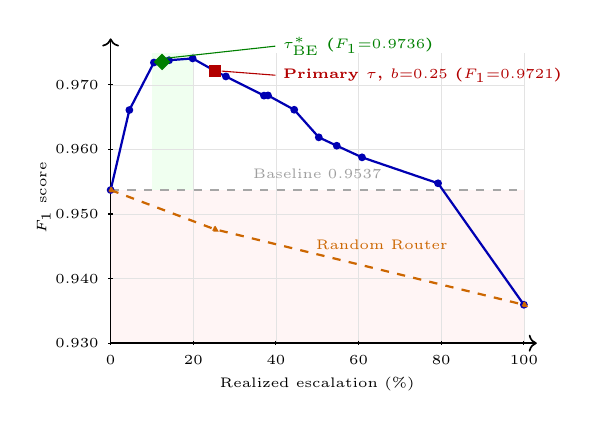
\begin{tikzpicture}[scale=0.82, every node/.style={font=\scriptsize}]
  % Subtle regime fills: collapse below baseline, high-gain ridge 10%--20%
  \fill[red!4] (0,0) rectangle (6.4,2.372);
  \fill[green!6] (0.64,2.372) rectangle (1.28,4.5);

  % Tick-aligned grid
  \foreach \x in {1.28, 2.56, 3.84, 5.12, 6.4}
    \draw[help lines, color=gray!22] (\x,0) -- (\x,4.5);
  \foreach \y in {1.0, 2.0, 3.0, 4.0}
    \draw[help lines, color=gray!22] (0,\y) -- (6.4,\y);

  % Axes
  \draw[->, semithick] (0,0) -- (6.60,0);
  \draw[->, semithick] (0,0) -- (0,4.72);

  % Ticks & titles
  \foreach \x/\val in {0/0, 1.28/20, 2.56/40, 3.84/60, 5.12/80, 6.4/100}
    \draw (\x,1pt) -- (\x,-1pt) node[below, font=\tiny] {\val};
  \foreach \y/\val in {0/0.930, 1.0/0.940, 2.0/0.950, 3.0/0.960, 4.0/0.970}
    \draw (1pt,\y) -- (-1pt,\y) node[left, font=\tiny] {\val};
  \node[below, font=\tiny] at (3.2,-0.38) {Realized escalation (\%)};
  \node[above, rotate=90, font=\tiny] at (-0.78,2.25) {$F_1$ score};

  % Specialist Baseline dashed line
  \draw[dashed, thick, color=gray!70] (0, 2.372) -- (6.4, 2.372);
  \node[above, font=\tiny, text=gray!75] at (3.20, 2.402) {Baseline $0.9537$};

  % Entropy frontier
  \draw[thick, color=blue!70!black, mark=*, mark size=1.2pt] plot coordinates {
    (0.000, 2.372) (0.290, 3.611) (0.670, 4.346) (0.905, 4.382) (1.270, 4.410) (1.619, 4.214) (1.785, 4.131) (2.375, 3.834) (2.437, 3.837) (2.843, 3.615) (3.224, 3.188) (3.502, 3.058) (3.893, 2.878) (5.071, 2.476) (6.400, 0.595)
  };

  % Primary tau (b = 0.25): square; tau*_BE: diamond
  \filldraw[red!70!black] (1.539, 4.134) rectangle (1.699, 4.294);
  \draw[red!70!black, thin] (1.719, 4.214) -- (2.55, 4.15);
  \node[right, font=\tiny\bfseries, text=red!70!black] at (2.52, 4.15) {Primary $\tau$, $b{=}0.25$ ($F_1{=}0.9721$)};
  \node[draw=green!50!black, fill=green!50!black, diamond, inner sep=1.4pt] at (0.796, 4.356) {};
  \draw[green!50!black, thin] (0.876, 4.416) -- (2.55, 4.6);
  \node[right, font=\tiny\bfseries, text=green!50!black] at (2.52, 4.6) {$\tau^{\ast}_{\mathrm{BE}}$ ($F_1{=}0.9736$)};

  % Random router
  \draw[thick, color=orange!80!black, dashed, mark=triangle*, mark size=1.2pt] plot coordinates {
    (0.000, 2.372) (1.609, 1.765) (6.400, 0.595)
  };
  \node[above, font=\tiny, text=orange!80!black] at (4.20, 1.30) {Random Router};
\end{tikzpicture}
\caption{Quality--cost frontier on E3 ($N=26{,}886$). $F_1$ reaches its ridge across
$10\%$--$20\%$ escalation, declines across the confident zone, and drops below the
specialist under full escalation. Square: $\tau$ ($b=0.25$); diamond:
$\tau^{\ast}_{\mathrm{BE}}$.}
\label{fig:frontier}
\end{figure}

\subsection{Cross-Vendor Generalization}
Collapse and recovery hold for all five models on the shared E9 benchmark
($N=3{,}000$, $\pi=4.83\%$; Table~\ref{tab:breakeven}). Under full escalation, every
LLM is significantly net-negative ($-69$ for Gemini to $-186$ for DeepSeek, all
$p<10^{-4}$) because measured intrusion ($\eps=6.58\%$--$9.98\%$) exceeds
$\epsstar=3.47\%$--$4.17\%$. Per corpus, the E3 pattern recurs for every model: full
escalation is net-positive only on PWD2021 ($+4$ to $+29$) and net-negative on
EBBU2017 and URL-Phish~2025 ($-2$ to $-162$).

Selective routing restores net gains for every vendor: at $\tau^{\ast}_{\mathrm{BE}}$
($11.3\%$ escalation), net rescues span $+42$ to $+75$, with every $95\%$ bootstrap
$F_1$ CI and every per-corpus cell strictly positive. At the wider $b=0.25$ budget
($24.6\%$), net gains span $+24$ to $+75$, with four of five $F_1$ CIs strictly above
zero. Consistent with the $\rrescue$-scaling of~\eqref{eq:breakeven}, the
lowest-rescue model, DeepSeek ($\rrescue=68.28\%$), incurs the largest
full-escalation loss ($-186$) and benefits most from tighter gating
($\tau^{\ast}_{\mathrm{BE}}$: $+42$, $\Delta F_1$ CI $[+0.0071,+0.0208]$ vs.\ $b=0.25$: $+24$, CI
$[-0.0012,+0.0163]$).

\subsection{Error Decomposition}
Full-escalation regressions disproportionately compromise security: on pooled E3, the
specialist confusion matrix
$(\mathit{TP},\mathit{FP},\mathit{FN},\mathit{TN})=(12{,}716,\,507,\,727,\,12{,}936)$
shifts to $(12{,}436,\,695,\,1{,}007,\,12{,}748)$ under full escalation. Missed
phishing rises by $280$ and false alarms by $188$, meaning $59.8\%$ of the $468$ net
added errors are phishing URLs the specialist had already caught, the higher-severity
SOC failure mode.

This asymmetry concentrates where corpus regularities are strongest
(Table~\ref{tab:cell_c}). On PWD2021, where $\eps<\epsstar$, escalation recovers
$204$ phishing URLs on net while adding only $7$ false alarms. On URL-Phish~2025,
full escalation drops $463$ phishing detections on net, and $78.2\%$ of its $734$
regressions are missed phishing. Among those $574$ missed-phishing regressions,
$98.95\%$ use \texttt{https://} ($91.1\%$ of all phishing vs.\ $33.9\%$ of legitimate
URLs) and $92.2\%$ carry nonempty paths (vs.\ $24.2\%$ of legitimate URLs).
Of these regressions, $97.6\%$ lie in the Bottom Zone at $\tau$ and $98.95\%$ at
$\tau^{\ast}_{\mathrm{BE}}$, so uncertainty routing keeps them on the local specialist.

\begin{table}[!t]
\caption{Error composition under full escalation on E3. Net columns: full-escalation
minus specialist counts; rightmost column: missed phishing as a share of regression
cell $C$ (pooled $853/1{,}439=59.3\%$ vs.\ $280/468=59.8\%$ of net added errors).}
\label{tab:cell_c}
\centering
\scriptsize
\setlength{\tabcolsep}{3.2pt}
\begin{tabular}{lrrrr}
\toprule
& \multicolumn{2}{c}{Net change under escalation} & & Missed phish. \\
\cmidrule(lr){2-3}
Corpus & Missed phishing & False alarms & $C$ & share of $C$ \\
\midrule
PWD2021 & $-204$ & $+7$ & 387 & $33.6\%$ \\
EBBU2017 & $+21$ & $+58$ & 318 & $46.9\%$ \\
URL-Phish 25 & $+463$ & $+123$ & 734 & $\mathbf{78.2\%}$ \\
\midrule
Pooled E3 \texttt{TEST} & $\mathbf{+280}$ & $\mathbf{+188}$ & 1{,}439 & $59.3\%$ \\
\bottomrule
\end{tabular}
\end{table}

\subsection{Latency and Cost}
At list price, Gemini~3.5 Flash-Lite averaged $375$ input and $63$ output tokens per
URL (\$271 per million URLs at full escalation); selective routing cuts this to
\$68.5 at $\tau$ and \$33.7 at $\tau^{\ast}_{\mathrm{BE}}$, while $74.7\%$--$87.6\%$
of traffic stays on the local CPU at sub-millisecond latency.

%==============================================================================
\section{Discussion and Limitations}
\label{sec:discussion}
%==============================================================================
\subsection{Deployment Guidance}
We recommend a three-step SOC rollout: (1)~estimate
$(\hat{\rrescue},\hat{\eps},\hat{\eps}^{\ast})$ on a labeled calibration sample of
$1{,}000$--$2{,}000$ URLs (pooled sign accuracy $98.9\%$--$100\%$, at least $91.8\%$
per corpus); (2)~whenever $\hat{\eps}>\hat{\eps}^{\ast}$, cap replace-on-escalation
inside the $10\%$--$25\%$ uncertainty head or tune $\tau^{\ast}_{\mathrm{BE}}$
directly on calibration data; and (3)~for wider cloud budgets, pair selective
routing with soft posterior fusion to suppress confident-zone regressions.

\subsection{Limitations}
Four limitations apply:
\emph{(i)~Modality and prompt:} triage operates on canonicalized URL strings under a
single zero-shot prompt without HTML, DNS, WHOIS, or specialist posterior context;
richer modalities may shift $(\rrescue,\eps)$.
\emph{(ii)~Model tiers and endpoints:} we test latency- and cost-matched cloud
tiers whose hosted snapshots evolve over time; larger frontier reasoning models
remain future work.
\emph{(iii)~Static corpora vs.\ live streams:} evaluation uses balanced public
benchmarks rather than nonstationary enterprise telemetry where class priors and
phishing campaigns drift continuously.
\emph{(iv)~Stochastic cloud decoding:} even with deterministic settings where
supported, repeated queries flip verdicts on $3.5\%$ of probed URLs, all in the
high-entropy stratum (Section~\ref{sec:setup}); strict reproducibility favors local
open-weight second tiers.

%==============================================================================
\section{Conclusion}
\label{sec:conclusion}
%==============================================================================
In high-accuracy phishing URL triage, the net gain of cloud LLM escalation is set by
the base-rate breakeven condition $\eps < \rrescue\,E/(N-E)$, not by LLM capability
alone. Unconstrained escalation lowers pooled $F_1$ from $0.9537$ to $0.9360$;
selective uncertainty routing lifts it to $0.9736$ at $12.45\%$ escalation, gains in
every corpus and vendor, and cuts list-price cost from \$271 to \$33.7 per million
URLs. Scripts, thresholds, prompts, ledgers, and anonymized caches are at
\url{https://github.com/FenitureMa/rivf2026-llm-url-routing}.

\section*{Acknowledgment}
Anthropic Claude and Google Gemini assisted with prose
editing and \LaTeX/TikZ formatting (Abstract, Sections~I--VII) and script/numerical
verification; all study design, analysis, and claims are the author's own, who
remains fully responsible for the manuscript.

\begin{thebibliography}{10}

\bibitem{sahingoz2019}
O.~K. Sahingoz, E.~Buber, O.~Demir, and B.~Diri, ``Machine learning based
phishing detection from URLs,'' \emph{Expert Syst.\ Appl.}, vol.~117,
pp.~345--357, 2019, doi: 10.1016/j.eswa.2018.09.029.

\bibitem{prasad2024}
A.~Prasad and S.~Chandra, ``PhiUSIIL: A diverse security profile empowered
phishing URL detection framework based on similarity index and incremental
learning,'' \emph{Comput.\ Secur.}, vol.~136, 2024, Art.\ no.~103545,
doi: 10.1016/j.cose.2023.103545.

\bibitem{sahoo2019}
D.~Sahoo, C.~Liu, and S.~C.~H. Hoi, ``Malicious URL detection using machine
learning: A survey,'' 2019, arXiv:1701.07179.

\bibitem{abdillah2023eval}
R.~Abdillah, Z.~Shukur, M.~Mohd, T.~S.~M.~Z. Murah, I.~Oh, and K.~Yim,
``Performance evaluation of phishing classification techniques on various data
sources and schemes,'' \emph{IEEE Access}, vol.~11, pp.~38721--38738, 2023,
doi: 10.1109/ACCESS.2022.3225971.

\bibitem{llmzeroshot2026}
N.~Hasan and P.~BusiReddyGari, ``Benchmarking large language models for zero-shot
and few-shot phishing URL detection,'' presented at the NeurIPS LAW Workshop, 2025, arXiv:2602.02641.

\bibitem{mdpi2025llm}
A.~H. Nasution, W.~Monika, A.~Onan, and Y.~Murakami, ``Benchmarking 21 open-source
large language models for phishing link detection with prompt engineering,''
\emph{Information}, vol.~16, no.~5, 2025, Art.\ no.~366,
doi: 10.3390/info16050366.

\bibitem{slm2025}
G.~Goldenits, P.~K\"{o}nig, S.~Raubitzek, and A.~Ekelhart, ``Small language models
for phishing website detection: Cost, performance, and privacy trade-offs,''
\emph{J.~Cybersecur.\ Priv.}, vol.~6, no.~2, 2026, Art.\ no.~48,
doi: 10.3390/jcp6020048.

\bibitem{clasp2025}
F.~Trad and A.~Chehab, ``CLASP: Cost-optimized LLM-based agentic system for phishing
detection,'' in \emph{Proc.\ 5th Int.\ Conf.\ Elect., Comput.\ Energy Technol.\
(ICECET)}, 2025, pp.~1--6, doi: \mbox{10.1109/}\allowbreak\mbox{ICECET63943.2025.11471974}.

\bibitem{ozaslan2026}
Y.~\"{O}zaslan and M.~F. Adak, ``A hybrid ML-LLM cascade system for cost-efficient
phishing webpage detection,'' in \emph{Proc.\ 10th Int.\ Young Eng.\ Forum Elect.\
Comput.\ Eng.\ (YEF-ECE)}, 2026, pp.~27--32,
doi: 10.1109/YEF-ECE70590.2026.11614634.

\bibitem{routingsurvey2026}
Y.~Moslem and J.~D. Kelleher, ``Dynamic model routing and cascading for efficient
LLM inference: A survey,'' \emph{Trans.\ Mach.\ Learn.\ Res.}, 2026,
arXiv:2603.04445.

\bibitem{ucci2026}
V.~Kotte, ``UCCI: Calibrated uncertainty for cost-optimal LLM cascade routing,''
2026, arXiv:2605.18796.

\bibitem{conformalcascade2026}
Y.~Dou, S.~Lian, and S.~Li, ``Conformal cascade: Distribution-free accuracy
guarantees for multi-tier LLM inference,'' 2026, arXiv:2607.25018.

\bibitem{geifman2017}
Y.~Geifman and R.~El-Yaniv, ``Selective classification for deep neural
networks,'' in \emph{Proc.\ Adv.\ Neural Inf.\ Process.\ Syst.\ (NeurIPS)},
vol.~30, 2017, pp.~4878--4887.

\bibitem{madras2018}
D.~Madras, T.~Pitassi, and R.~Zemel, ``Predict responsibly: Improving fairness
and accuracy by learning to defer,'' in \emph{Proc.\ Adv.\ Neural Inf.\ Process.\
Syst.\ (NeurIPS)}, vol.~31, 2018, pp.~6147--6157.

\bibitem{jitkrittum2023}
W.~Jitkrittum, N.~Gupta, A.~K. Menon, H.~Narasimhan, A.~S. Rawat, and
S.~Kumar, ``When does confidence-based cascade deferral suffice?'' in
\emph{Proc.\ Adv.\ Neural Inf.\ Process.\ Syst.\ (NeurIPS)}, vol.~36, 2023,
pp.~9891--9906, doi: 10.52202/075280-0431.

\bibitem{ariyadasa2021dataset}
S.~Ariyadasa, ``Phishing websites dataset,'' Mendeley Data, 2021,
doi: 10.17632/n96ncsr5g4.1.

\bibitem{linh2025dataset}
D.~M. Linh and T.~C. Hung, ``URL-Phish: A feature-engineered dataset for
phishing detection,'' Mendeley Data, 2025, doi: 10.17632/65z9twcx3r.1.

\end{thebibliography}

\end{document}
